% Created 2021-09-11 Sat 16:43
% Intended LaTeX compiler: xelatex
\documentclass[letterpaper]{article}
\usepackage{graphicx}
\usepackage{grffile}
\usepackage{longtable}
\usepackage{wrapfig}
\usepackage{rotating}
\usepackage[normalem]{ulem}
\usepackage{amsmath}
\usepackage{textcomp}
\usepackage{amssymb}
\usepackage{capt-of}
\usepackage{hyperref}
\usepackage[margin=1in]{geometry}
\usepackage{fontspec}
\usepackage{indentfirst}
\setmainfont[ItalicFont = LiberationSans-Italic, BoldFont = LiberationSans-Bold, BoldItalicFont = LiberationSans-BoldItalic]{LiberationSans}
\newfontfamily\NHLight[ItalicFont = LiberationSansNarrow-Italic, BoldFont       = LiberationSansNarrow-Bold, BoldItalicFont = LiberationSansNarrow-BoldItalic]{LiberationSansNarrow}
\newcommand\textrmlf[1]{{\NHLight#1}}
\newcommand\textitlf[1]{{\NHLight\itshape#1}}
\let\textbflf\textrm
\newcommand\textulf[1]{{\NHLight\bfseries#1}}
\newcommand\textuitlf[1]{{\NHLight\bfseries\itshape#1}}
\usepackage{fancyhdr}
\pagestyle{fancy}
\usepackage{titlesec}
\usepackage{titling}
\makeatletter
\lhead{\textbf{\@title}}
\makeatother
\rhead{\textrmlf{Compiled} \today}
\lfoot{\theauthor\ \textbullet \ \textbf{2021-2022}}
\cfoot{}
\rfoot{\textrmlf{Page} \thepage}
\titleformat{\section} {\Large} {\textrmlf{\thesection} {|}} {0.3em} {\textbf}
\titleformat{\subsection} {\large} {\textrmlf{\thesubsection} {|}} {0.2em} {\textbf}
\titleformat{\subsubsection} {\large} {\textrmlf{\thesubsubsection} {|}} {0.1em} {\textbf}
\setlength{\parskip}{0.45em}
\renewcommand\maketitle{}
\author{Houjun Liu}
\date{\today}
\title{Deravitaves}
\hypersetup{
 pdfauthor={Houjun Liu},
 pdftitle={Deravitaves},
 pdfkeywords={},
 pdfsubject={},
 pdfcreator={Emacs 27.2 (Org mode 9.4.4)}, 
 pdflang={English}}
\begin{document}

\maketitle


\section{Derivatives}
\label{sec:orgdfd4ce2}
=> Instantaneous rate of change at a particular point

\begin{itemize}
\item Average rate of change = \(\frac{\Delta Y}{\Delta X}\)
\end{itemize}

\begin{figure}[htbp]
\centering
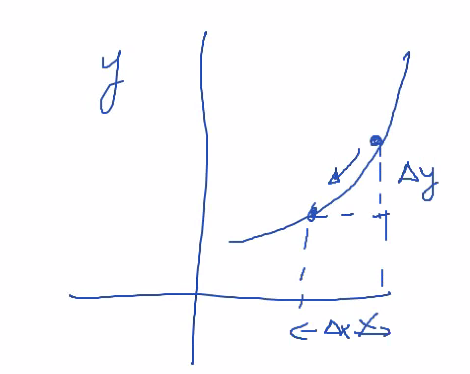
\includegraphics[width=.9\linewidth]{rateofchange.png}
\caption{rateofchange.png}
\end{figure}

\begin{itemize}
\item Instantaneous rate of change =
\(\lim_{\Delta x \to 0} \frac{\Delta Y}{\Delta X}\)
\end{itemize}

Derivative of \(f(x)\) => \(\frac{dy}{dx}\)

\begin{figure}[htbp]
\centering
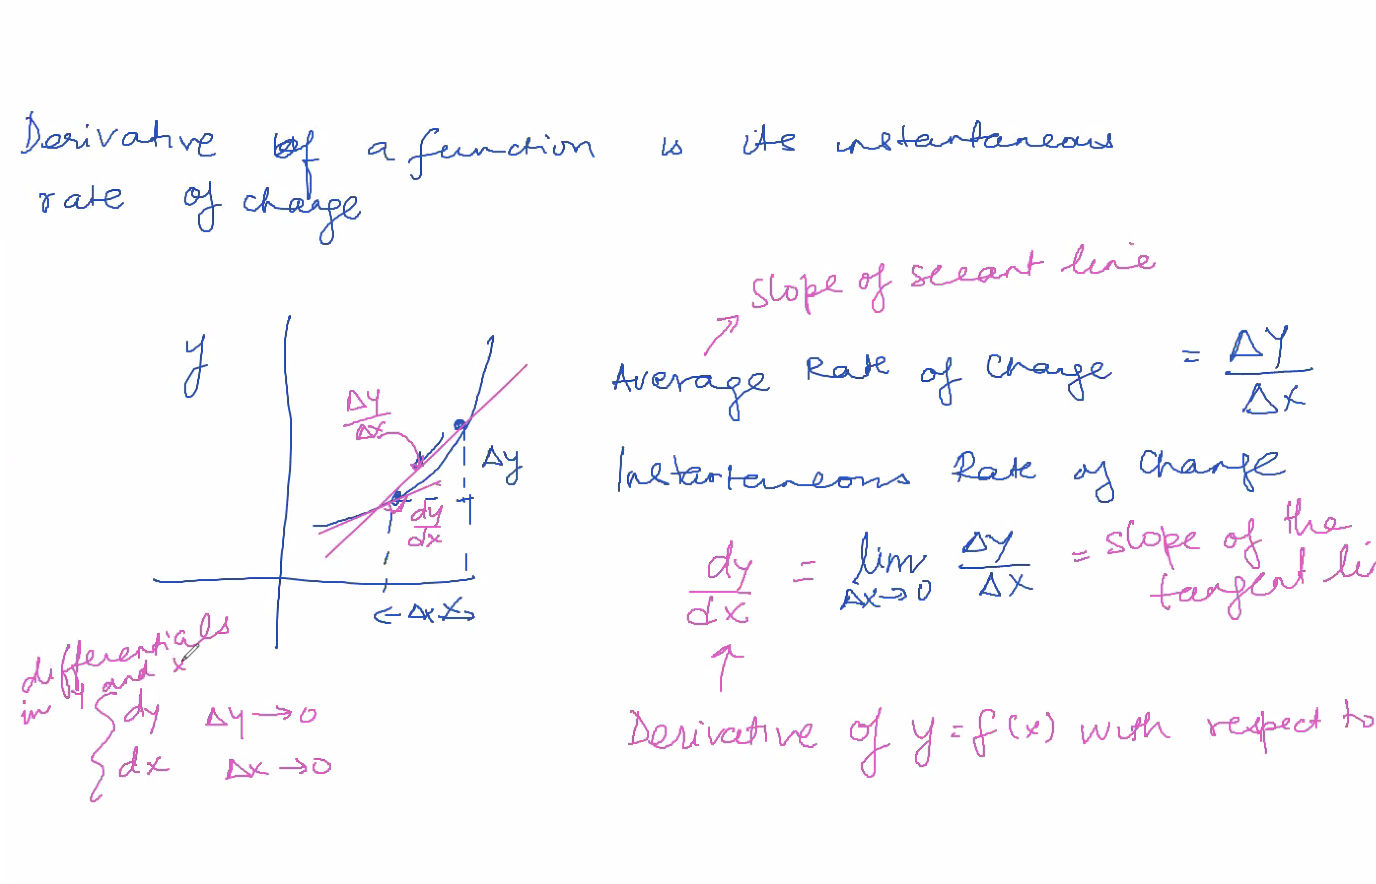
\includegraphics[width=.9\linewidth]{derivativesWB.png}
\caption{derivativesWB.png}
\end{figure}

\subsection{Useful Table of Derivatives}
\label{sec:org1f98166}
\begin{center}
\begin{tabular}{ll}
f(x) & f'(x)\\
\hline
\(x^2\) & \(2x\)\\
\(x^3\) & \(3x^2\)\\
\(x^n\) & \(nx^{n-1}\)\\
\(\frac{1}{x}\) & \(\frac{-1}{x^2}\)\\
\(\sqrt{x}\) & \(\frac{1}{2 \sqrt{x}}\)\\
\(\sin(x)\) & \(\cos (x)\)\\
\(\cos(x)\) & \(-\sin (x)\)\\
\(\tan(x)\) & \(1 + \tan^2 (x) = sec^2(x)\)\\
\(\cot(x)\) & \(-\csc^2 (x)\)\\
\(\sec(x)\) & \(\tan(x) \sec(x)\)\\
\(\csc(x)\) & \(-\cot(x) \csc(x)\)\\
\(e^x\) & \(e^x\)\\
\(ln(x)\) & \(\frac{1}{x}\)\\
\(a^x\) & \(a^x ln(a)\)\\
\(log_a(x)\) & \(\frac{1}{x ln(a)}\)\\
\(f^-1(x)\) & \(\frac{1}{f'(f^-1(x))}\)\\
\(sin^-1(ax)\) & \(\frac{a}{\sqrt{1-(ax)^2}}\)\\
\(cos^-1(ax)\) & \(\frac{-1}{\sqrt{1-(ax)^2}}\)\\
\(tan^-1(ax)\) & \(\frac{1}{1+(ax)^2}\)\\
\end{tabular}
\end{center}
\end{document}
